% ============================================================
% 原文第 1-16 页（第 1 页文档标题与作者信息已在主文件处理）
% ============================================================

\section{作业总览}

在本作业中，你将构建训练一个标准 Transformer 语言模型（language model，LM）所需的全部组件，并训练若干模型。

\textbf{你将实现的内容}
\begin{enumerate}
  \item 字节对编码（byte-pair encoding，BPE）分词器（见第 2 节）
  \item Transformer 语言模型（LM）（见第 3 节）
  \item 交叉熵损失函数与 AdamW 优化器（见第 4 节）
  \item 训练循环，支持模型与优化器状态的序列化保存和加载（见第 5 节）
\end{enumerate}

\textbf{你将运行的内容}
\begin{enumerate}
  \item 在 TinyStories 数据集上训练 BPE 分词器。
  \item 用训练好的分词器对数据集进行编码，把它转换为整数 ID 序列。
  \item 在 TinyStories 数据集上训练 Transformer 语言模型。
  \item 使用训练好的 Transformer 语言模型进行样本生成与困惑度（perplexity）评估。
  \item 在 OpenWebText 上训练模型，并把你取得的困惑度提交到排行榜（leaderboard）。
\end{enumerate}

\textbf{你可以使用的内容}

我们期望你从零开始构建每个组件。特别地，除非属于下面列出的内容，你不得使用 \tm{torch.nn}、\tm{torch.nn.functional} 或 \tm{torch.optim} 中的任何定义：
\begin{itemize}
  \item \tm{torch.nn.Parameter}
  \item \tm{torch.nn} 中的容器类（例如 \tm{Module}、\tm{ModuleList}、\tm{Sequential} 等）。\footnote{完整列表见 \url{pytorch.org/docs/stable/nn.html\#containers}。}
  \item \tm{torch.optim.Optimizer} 基类
\end{itemize}

除此之外的任何 PyTorch 定义你都可以使用。如果你想使用某个函数或类，但不确定它是否被允许，欢迎随时在 Slack 上提问。拿不准的时候，请思考一下：使用它是否会损害本作业"从零实现"的初衷。

\textbf{关于 AI 工具的声明}

AI 可以完全自主地解决作业中的许多部分。这使得深入投入课程材料并从中学习变得更加困难。

允许将 AI 工具用于回答高层次的概念性问题，或提供低层次的编程文档（例如函数签名、库 API）。但是，不允许用 AI 工具实现作业的任何部分。这既包括编码智能体（例如 Cursor Agents、Codex、Claude Code），也包括 AI 自动补全（例如 Cursor Tab、GitHub Copilot）。使用 AI 智能体时，请确保它使用随作业提供的 \tm{AGENTS.md} 文件；使用聊天机器人时，也请附上你使用的提示词（prompt）。

我们强烈建议你在完成作业时在 IDE 中禁用 AI 自动补全（例如 Cursor Tab、GitHub Copilot）（不过非 AI 的自动补全，例如函数名自动补全，完全没有问题）。往届同学特别提到，禁用 AI 自动补全让他们更容易深入理解课程内容。

完整的 AI 政策请参见这份文档（链接见原文）。

\textbf{代码是什么样的}

作业代码以及本说明文档都发布在 GitHub 上：

\begin{center}
\url{github.com/stanford-cs336/assignment1-basics}
\end{center}

请 \tm{git clone} 该仓库。如果仓库有更新，我们会通知你，届时你 \tm{git pull} 即可获得最新内容。
\begin{enumerate}
  \item \tm{cs336\_basics/*}：这是你写代码的地方。注意这里面没有任何代码——你完全可以从零开始自由发挥！
  \item \tm{adapters.py}：这里定义了你的代码必须提供的一组功能。对于每一项功能（例如缩放点积注意力），请在对应的实现函数（例如 \tm{run\_scaled\_dot\_product\_attention}）里直接调用你自己的代码来完成填充。注意：你对 \tm{adapters.py} 的修改不应包含任何实质性逻辑；它只是胶水代码。
  \item \tm{test\_*.py}：这里包含你必须通过的全部测试（例如 \tm{test\_scaled\_dot\_product\_attention}），这些测试会调用 \tm{adapters.py} 中定义的钩子（hook）。请不要编辑测试文件。
\end{enumerate}

\textbf{如何提交}

要提交，请运行 \tm{make\_submission.sh} 生成提交用的 zip 文件。如果你有不希望包含在提交 zip 里的较大数据文件或 checkpoint，请务必把它们添加到脚本中的排除列表。

你需要在 Gradescope 上提交以下文件：
\begin{itemize}
  \item \tm{writeup.pdf}：回答所有书面问题。请对你的回答进行排版。
  \item \tm{code.zip}：包含你编写的全部代码。
\end{itemize}

要提交到排行榜，请向以下仓库提交 PR：

\begin{center}
\url{github.com/stanford-cs336/assignment1-basics-leaderboard}
\end{center}

详细的提交说明见排行榜仓库中的 \tm{README.md}。

\textbf{从哪里获取数据集}

本作业将使用两个预处理数据集：TinyStories [R.~Eldan et al., 2023] 与 OpenWebText [A.~Gokaslan et al., 2019]。这两个数据集都是单个的大型纯文本文件。

如果你是随课程一起完成本作业，可以在 compute guide 中找到数据集的下载说明。

如果你是在家自学，可以使用 \tm{README.md} 中的命令下载这些文件。

\textbf{低资源提示：初始化（Init）}

在本课程的各次作业说明中，我们会给出在较少乃至没有 GPU 资源的情况下完成作业的建议。例如，我们有时会建议\textbf{缩减规模}（downscaling）你的数据集或模型大小，或者讲解如何在 Mac 的集成 GPU 或 CPU 上运行训练代码。你会在这类蓝色方框中看到这些"低资源提示"。即便是可以使用课程机器的斯坦福在校生，这些提示也可能帮助你更快地迭代并节省时间，因此我们建议阅读它们！

\textbf{低资源提示：在 Apple Silicon 或 CPU 上完成作业 1}

使用助教（staff）的参考解答代码，我们可以在配备 36 GB 内存的 Apple M4 Max 芯片上训练出一个能生成相当流畅文本的 LM：在 Metal GPU（MPS）上用时不到 5 分钟，用 CPU 大约 30 分钟。如果这些说法对你来说没什么概念，别担心！你只需要知道：只要你的笔记本电脑还算新，且你的实现正确而高效，你就能训练出一个能以不错的流畅度生成简单儿童故事的小型 LM。

在作业后面的部分，我们会说明如果你使用的是 CPU 或 MPS，需要做哪些改动。

\section{字节对编码（BPE）分词器}

在作业的第一部分，我们将训练并实现一个字节级的字节对编码（BPE）分词器 [R.~Sennrich et al., 2016; C.~Wang et al., 2019]。具体来说，我们会把任意（Unicode）字符串表示为字节序列，并在该字节序列上训练 BPE 分词器。之后，我们会用这个分词器把文本（字符串）编码为 token（整数序列），用于语言建模。

\subsection{Unicode 标准}

Unicode 是一种文本编码标准，它把字符映射为整数码点（code point）。截至 Unicode 17.0（2025 年 9 月发布），该标准在 172 个文字系统（script）中定义了 159,801 个字符。例如，字符 "s" 的码点是 115（通常记作 U+0073，其中 U+ 是约定前缀，0073 是 115 的十六进制表示），而字符 "牛" 的码点是 29275。在 Python 中，你可以用 \tm{ord()} 函数把单个 Unicode 字符转换为它的整数表示；\tm{chr()} 函数则把一个整数 Unicode 码点转换为含有对应字符的字符串。

\begin{lstlisting}
>>> ord('牛')
29275
>>> chr(29275)
'牛'
\end{lstlisting}

\subsubsection*{问题（\tm{unicode1}）：理解 Unicode（1 分）}

\begin{enumerate}[label=(\alph*)]
  \item \tm{chr(0)} 返回的是什么 Unicode 字符？

        \textbf{交付要求}：一句话回答。

  \item 这个字符的字符串表示（\tm{\_\_repr\_\_()}）与它的打印（print）表示有什么不同？

        \textbf{交付要求}：一句话回答。

  \item 当这个字符出现在文本中时会发生什么？你可以在 Python 解释器里试着运行下面的代码，看看结果是否符合你的预期：

\begin{lstlisting}
>>> chr(0)
>>> print(chr(0))
>>> "this is a test" + chr(0) + "string"
>>> print("this is a test" + chr(0) + "string")
\end{lstlisting}

        \textbf{交付要求}：一句话回答。
\end{enumerate}

\subsection{Unicode 编码}

虽然 Unicode 标准定义了从字符到码点（整数）的映射，但直接在 Unicode 码点上训练分词器并不现实：这样的词表会过于庞大（约 15 万项）且稀疏（许多字符都非常罕见）。因此我们改用 Unicode 编码（Unicode encoding），它把一个 Unicode 字符转换为字节序列。Unicode 标准本身定义了三种编码：UTF-8、UTF-16 和 UTF-32，其中 UTF-8 是互联网上的主导编码（超过 98\% 的网页都在使用）。

要把 Unicode 字符串编码为 UTF-8，可以使用 Python 的 \tm{encode()} 函数。要访问 Python \tm{bytes} 对象的底层字节值，可以对其进行迭代（例如调用 \tm{list()}）。最后，可以用 \tm{decode()} 函数把 UTF-8 字节串解码为 Unicode 字符串。

\begin{lstlisting}
>>> test_string = "hello! こんにちは!"
>>> utf8_encoded = test_string.encode("utf-8")
>>> print(utf8_encoded)
b'hello! \xe3\x81\x93\xe3\x82\x93\xe3\x81\xab\xe3\x81\xa1\xe3\x81\xaf!'
>>> print(type(utf8_encoded))
<class 'bytes'>
>>> # 取得编码后字符串的字节值（0 到 255 的整数）。
>>> list(utf8_encoded)
[104, 101, 108, 108, 111, 33, 32, 227, 129, 147, 227, 130, 147, 227, 129, 171, 227, 129,
161, 227, 129, 175, 33]
>>> # 一个字节并不一定对应一个 Unicode 字符！
>>> print(len(test_string))
13
>>> print(len(utf8_encoded))
23
>>> print(utf8_encoded.decode("utf-8"))
hello! こんにちは!
\end{lstlisting}

把 Unicode 码点转换为字节序列（例如通过 UTF-8 编码）后，我们实际上是把一个码点序列（21 位整数，其中有 159,801 个有效值）转换成了一个字节值序列（0 到 255 范围内的整数）。长度为 256 的字节词表处理起来要容易得多。使用字节级分词（byte-level tokenization）时，我们不需要担心词表外（out-of-vocabulary）token，因为我们知道任何输入文本都可以表示为 0 到 255 的整数序列。

\subsubsection*{问题（\tm{unicode2}）：Unicode 编码（3 分）}

\begin{enumerate}[label=(\alph*)]
  \item 相比 UTF-16 或 UTF-32，为什么更倾向于在 UTF-8 编码的字节上训练我们的分词器？比较这些编码对各种输入字符串的输出可能会对你有所帮助。

        \textbf{交付要求}：一到两句话回答。

  \item 考虑下面这个（不正确的）函数，它的本意是把 UTF-8 字节串解码为 Unicode 字符串。这个函数为什么是不正确的？请给出一个会产生错误结果的输入字节串示例。

\begin{lstlisting}
def decode_utf8_bytes_to_str_wrong(bytestring: bytes):
    return "".join([bytes([b]).decode("utf-8") for b in bytestring])

>>> decode_utf8_bytes_to_str_wrong("hello".encode("utf-8"))
'hello'
\end{lstlisting}

        \textbf{交付要求}：给出一个使 \tm{decode\_utf8\_bytes\_to\_str\_wrong} 产生错误输出的输入字节串示例，并用一句话解释该函数为什么是不正确的。

  \item 给出一个无法解码为任何 Unicode 字符的两字节序列。

        \textbf{交付要求}：给出一个示例，并用一句话解释。
\end{enumerate}

\subsection{子词分词}

字节级分词虽然能缓解词级分词器面临的词表外问题，但把文本切分为字节会导致输入序列极长。这会拖慢模型训练：一个含 10 个单词的句子在词级语言模型中可能只有 10 个 token 长，而在字符级模型中可能有 50 个甚至更多 token（取决于单词的长度）。处理这些更长的序列需要模型在每一步进行更多计算。此外，在字节序列上做语言建模也很困难，因为更长的输入序列会在数据中引入长程依赖。

子词分词（subword tokenization）是介于词级分词器与字节级分词器之间的一种折中。注意，字节级分词器的词表有 256 个条目（字节取值为 0 到 255）。子词分词器以更大的词表规模换取对输入字节序列更好的压缩。例如，如果字节序列 \tm{b'the'} 在我们的原始文本训练数据中频繁出现，就在词表中为它分配一个条目，这样这个 3-token 序列就可以缩减为单个 token。

我们如何挑选这些要加入词表的子词单元？R.~Sennrich et al.~[3] 提出使用字节对编码（BPE；P.~Gage [5]），它是一种压缩算法，迭代地用一个新的、未被使用的索引来替换（"合并"）出现频率最高的字节对。注意，该算法通过向词表添加子词 token 来最大化输入序列的压缩——只要一个词在输入文本中出现得足够频繁，它最终就会被表示为单个子词单元。

词表通过 BPE 构建的子词分词器通常称为 BPE 分词器。在本作业中，我们将实现一个字节级 BPE 分词器，其词表条目是字节或合并后的字节序列，这在词表外处理与可控的输入序列长度两方面兼得。构建 BPE 分词器词表的过程称为"训练"BPE 分词器。

\subsection{BPE 分词器的训练}

BPE 分词器的训练流程包括三个主要步骤。

\textbf{词表初始化}

分词器词表是从字节串（bytestring）token 到整数 ID 的一一映射。由于我们训练的是字节级 BPE 分词器，初始词表就是全部字节的集合。因为字节取值共有 256 种，所以初始词表的大小为 256。

\textbf{预分词}

有了词表之后，原则上你可以直接统计文本中各字节相邻出现的频率，并从最高频的字节对开始合并。然而这在计算上相当昂贵，因为每合并一次都要对语料库做一次完整扫描。此外，直接在整个语料库上跨边界合并字节，可能产生仅标点不同的 token（例如 \tm{dog!} 与 \tm{dog.}）。这些 token 会被赋予完全不同的 token ID，尽管它们很可能具有很高的语义相似性（因为它们只差一个标点）。

为了避免这一点，我们对语料库进行预分词（pre-tokenize）。你可以把它理解为对语料库的一种粗粒度分词，它帮助我们统计字符对出现的频率。例如，单词 'text' 可能是出现了 10 次的一个预分词（pre-token）。这样，当我们统计字符 't' 和 'e' 相邻出现的次数时，会发现单词 'text' 中 't' 与 'e' 相邻，于是可以把它们的计数直接加 10，而不必翻查整个语料库。由于我们训练的是字节级 BPE 模型，每个预分词都被表示为一个 UTF-8 字节序列。

R.~Sennrich et al.~[3] 的原始 BPE 实现直接按空白切分来预分词（即 \tm{s.split(" ")}）。基于 SentencePiece 的分词器（例如 Llama 1 和 2 的分词器）至今仍在使用这种方法。

大多数现代分词器使用基于正则表达式的预分词器，这一做法源自 GPT-2；A.~Radford et al.~[6]。我们将使用原始正则的一个略加修饰的版本，取自
\url{github.com/openai/tiktoken/pull/234/files}：

\begin{lstlisting}
>>> PAT = r"""'(?:[sdmt]|ll|ve|re)| ?\p{L}+| ?\p{N}+| ?[^\s\p{L}\p{N}]+|\s+(?!\S)|\s+"""
\end{lstlisting}

用这个预分词器交互式地切分一些文本，或许有助于你更好地理解它的行为：

\begin{lstlisting}
>>> # 需要 `regex` 包
>>> import regex as re
>>> re.findall(PAT, "some text that i'll pre-tokenize")
['some', ' text', ' that', ' i', "'ll", ' pre', '-', 'tokenize']
\end{lstlisting}

不过在代码中使用它时，你应当使用 \tm{re.finditer}，以免在构建"预分词 $\to$ 计数"的映射时把这些预分词得到的词都存储下来。

\textbf{计算 BPE 合并}

现在我们已经把输入文本转换为预分词，并把每个预分词表示为 UTF-8 字节序列，接下来就可以计算 BPE 合并（即训练 BPE 分词器）了。概括地说，BPE 算法迭代地统计每一对字节，并找出频率最高的对（"A", "B"）。随后，这个最高频对（"A", "B"）的每一处出现都会被合并，即替换为新 token "AB"。这个新合并出的 token 会被加入词表；因此 BPE 训练结束后的最终词表大小等于初始词表大小（在我们的设定中为 256）加上训练期间执行的 BPE 合并次数。为了提高 BPE 训练效率，我们不考虑跨越预分词边界的字节对。\footnote{注意，R.~Sennrich et al.~[3] 的原始 BPE 公式规定要引入词尾（end-of-word）token。我们训练字节级 BPE 模型时不添加词尾 token，因为所有字节（包括空白和标点）都已包含在模型词表中。既然我们已经显式地表示了空格和标点，学到的 BPE 合并自然会反映出这些词边界。}在计算合并时，如果字节对的频率出现并列，则确定性地偏向字典序（lexicographically）更大的对。例如，如果（"A", "B"）、（"A", "C"）、（"B", "ZZ"）和（"BA", "A"）都具有最高频率，我们会合并（"BA", "A"）：

\begin{lstlisting}
>>> max([("A", "B"), ("A", "C"), ("B", "ZZ"), ("BA", "A")])
('BA', 'A')
\end{lstlisting}

\textbf{特殊 token}

有些字符串（例如 \tm{<|endoftext|>}）常被用来编码元数据（例如文档之间的边界）。在编码文本时，通常需要把某些字符串当作"特殊 token"（special tokens）对待：它们永远不应被切分成多个 token（即始终保留为单个 token）。例如，序列结束字符串 \tm{<|endoftext|>} 应当始终保留为单个 token（即单个整数 ID），这样我们才知道什么时候应停止语言模型的生成。这些特殊 token 必须加入词表，从而拥有对应的固定 token ID。

R.~Sennrich et al.~[3] 的算法 1 给出了一个低效的 BPE 分词器训练实现（基本遵循我们上面概述的步骤）。作为第一个练习，实现并测试这个函数或许有助于检验你的理解。

\subsubsection*{示例（\tm{bpe\_example}）：BPE 训练示例}

这是取自 R.~Sennrich et al.~[3] 的一个风格化示例。考虑一个由以下文本构成的语料库

\begin{lstlisting}
low low low low low
lower lower widest widest widest
newest newest newest newest newest newest
\end{lstlisting}

并且词表中有一个特殊 token \tm{<|endoftext|>}。

\textbf{词表}

我们用特殊 token \tm{<|endoftext|>} 和 256 个字节值来初始化词表。

\textbf{预分词}

为了简单起见，也为了聚焦合并过程，本示例假设预分词就是按空白切分。预分词并计数后，我们得到如下频率表：

\begin{lstlisting}
{low: 5, lower: 2, widest: 3, newest: 6}
\end{lstlisting}

把它表示为 \tm{dict[tuple[bytes, ...], int]} 会很方便，例如 \tm{\{(l,o,w): 5, ...\}}。注意，即便单个字节在 Python 中也是一个 \tm{bytes} 对象。Python 中没有用来表示单个字节的 \tm{byte} 类型，正如没有用来表示单个字符的 \tm{char} 类型一样。

\textbf{合并}

我们先考察每一对相邻字节，并对它们出现的词的频率求和：\tm{\{lo: 7, ow: 7, we: 8, er: 2, wi: 3, id: 3, de: 3, es: 9, st: 9, ne: 6, ew: 6\}}。字节对 ('e', 's') 与 ('s', 't') 频率并列，因此我们取字典序更大的 ('s', 't')。接着我们合并预分词，得到 \tm{\{(l,o,w): 5, (l,o,w,e,r): 2, (w,i,d,e,st): 3, (n,e,w,e,st): 6\}}。

第二轮中，我们发现 (e, st) 是最常见字节对（计数为 9），将其合并后得到 \tm{\{(l,o,w): 5, (l,o,w,e,r): 2, (w,i,d,est): 3, (n,e,w,est): 6\}}。依此继续，最终得到的合并序列为 \tm{['s t', 'e st', 'o w', 'l ow', 'w est', 'n e', 'ne west', 'w i', 'wi d', 'wid est', 'low e', 'lowe r']}。

如果我们只做 6 次合并，得到 \tm{['s t', 'e st', 'o w', 'l ow', 'w est', 'n e']}，此时词表条目为 \tm{[<|endoftext|>, [...256 BYTE CHARS], st, est, ow, low, west, ne]}。

使用这个词表和这组合并，单词 newest 会被分词为 \tm{[ne, west]}。

\subsection{BPE 分词器训练实验}

让我们在 TinyStories 数据集上训练一个字节级 BPE 分词器。数据集的查找/下载说明见第 1 节。在开始之前，我们建议先浏览一下 TinyStories 数据集，了解其中的数据大概是什么样子。

\textbf{并行化预分词}

你会发现预分词步骤是一个主要瓶颈。可以使用内置库 \tm{multiprocessing} 对代码进行并行化来加速预分词。具体来说，我们建议在并行实现预分词时对语料库分块，并确保块边界落在某个特殊 token 的开头。你可以原封不动地使用下面链接中的起始代码来获得块边界，然后用它把工作分配到你的各个进程：

\begin{center}
\url{https://github.com/stanford-cs336/assignment1-basics/blob/main/cs336_basics/pretokenization_example.py}
\end{center}

这种分块总是有效的，因为我们从不希望跨越文档边界进行合并。就本作业而言，你始终可以这样切分。不必担心收到一个不含 \tm{<|endoftext|>} 的超大语料库这种边缘情况。

\textbf{预分词前移除特殊 token}

在用正则模式运行预分词（使用 \tm{re.finditer}）之前，你应当先把语料库（如果采用并行实现，则是你的分块）中的所有特殊 token 剔除。请确保按特殊 token 进行切分，使任何合并都不会跨越它们所界定的文本。例如，如果你的语料库（或分块）形如 \tm{[Doc 1]<|endoftext|>[Doc 2]}，你应当按特殊 token \tm{<|endoftext|>} 切分，再分别对 \tm{[Doc 1]} 和 \tm{[Doc 2]} 预分词，这样合并就不会跨越文档边界。换句话说，特殊 token 在训练期间定义了硬性的分段边界，但它们本身不应计入合并统计。这可以通过 \tm{re.split} 并以 \tm{"|".join(special\_tokens)} 作为分隔符来实现（注意小心使用 \tm{re.escape}，因为特殊 token 中可能出现 | 字符）。测试 \tm{test\_train\_bpe\_special\_tokens} 会检验这一点。

\textbf{优化合并步骤}

上面风格化示例中的朴素 BPE 训练实现之所以慢，是因为每做一次合并，它都要遍历所有字节对来找出最高频对。然而，每次合并后发生变化的，只有与被合并对相重叠的那些对的计数。因此，通过为所有字节对的计数建立索引并增量更新这些计数（而不是显式遍历每一对字节来统计频率），可以提升 BPE 训练的速度。这一缓存手段能带来显著的加速，不过我们要指出，BPE 训练中的合并部分在 Python 中是\textbf{无法}并行的。

\textbf{低资源提示：性能分析（Profiling）}

你应当使用 \tm{cProfile} 或 \tm{py-spy} 之类的性能分析工具找出你实现中的瓶颈，并集中优化那些部分。

\textbf{低资源提示："缩减规模"（Downscaling）}

与其一上来就在完整的 TinyStories 数据集上训练分词器，我们建议你先在一个小的数据子集（"调试数据集"）上训练。例如，你可以改在 TinyStories 验证集上训练分词器——它只有 22K 个文档，而不是 2.12M 个。这体现了一条通用策略：尽可能缩减规模来加速开发，例如使用更小的数据集、更小的模型规模等。选择调试数据集或超参数配置的规模需要仔细权衡：你希望调试集足够大，能够暴露与完整配置相同的瓶颈（这样你所做的优化才能推广到完整配置），但又不能大到运行起来没完没了。

\subsubsection*{问题（\tm{train\_bpe}）：BPE 分词器训练（15 分）}

\textbf{交付要求}：编写一个函数，给定输入文本文件的路径，训练一个（字节级）BPE 分词器。你的 BPE 训练函数应至少能处理以下输入参数：

\textbf{输入}
\begin{description}
  \item[\tm{input\_path: str}] 存放 BPE 分词器训练数据的文本文件路径。
  \item[\tm{vocab\_size: int}] 一个正整数，定义最终词表的最大尺寸（包括初始字节词表、由合并产生的词表条目以及任何特殊 token）。
  \item[\tm{special\_tokens: list[str]}] 要加入词表的字符串列表。训练期间，把它们视为硬边界，阻止跨越其跨度的合并；但在计算合并统计时不要把它们包含在内。
\end{description}

你的 BPE 训练函数应返回得到的词表和合并：

\textbf{输出}
\begin{description}
  \item[\tm{vocab: dict[int, bytes]}] 分词器词表，即从 \tm{int}（词表中的 token ID）到 \tm{bytes}（token 字节）的映射。
  \item[\tm{merges: list[tuple[bytes, bytes]]}] 训练产生的 BPE 合并列表。列表的每个元素是一个字节元组 \tm{(<token1>, <token2>)}，表示 \tm{<token1>} 与 \tm{<token2>} 发生了合并。合并应按创建顺序排列。
\end{description}

要用我们提供的测试来检验你的 BPE 训练函数，你需要先实现 \tm{[adapters.run\_train\_bpe]} 处的测试适配器，然后运行 \tm{uv run pytest tests/test\_train\_bpe.py}。你的实现应能通过所有测试。可选地（这可能需要投入大量时间），你可以用某种系统级语言来实现训练方法的关键部分，例如 C++（考虑 \tm{cppyy} 或 \tm{nanobind}）或 Rust（使用 PyO3）。如果这样做，请注意哪些操作需要复制数据、哪些操作可以直接读取 Python 内存，并确保留下构建说明，或者确保仅凭 \tm{pyproject.toml} 就能完成构建。另外请注意，GPT-2 正则表达式在大多数正则引擎中支持不佳，而且在多数支持它的引擎中会很慢。我们验证过 Oniguruma 速度尚可且支持负向前瞻（negative lookahead），不过如果说有什么差别，Python 的 \tm{regex} 包甚至更快。

\subsubsection*{问题（\tm{train\_bpe\_tinystories}）：在 TinyStories 上进行 BPE 训练（2 分）}

\begin{enumerate}[label=(\alph*)]
  \item 在 TinyStories 数据集上训练一个字节级 BPE 分词器，最大词表规模取 10,000。确保把 TinyStories 的特殊 token \tm{<|endoftext|>} 加入词表。把得到的词表和合并序列化保存到磁盘，以供进一步检查。训练花费了多少时间和内存？词表中最长的 token 是什么？它合理吗？

        \textbf{资源需求}：$\leq$ 30 分钟（无 GPU）；$\leq$ 30 GB 内存

        \textbf{提示}：在预分词阶段使用 \tm{multiprocessing} 并行化，并利用下面两个事实，你应该能把 BPE 训练的时间控制在 2 分钟以内：
        \begin{enumerate}[label=(\alph*)]
          \item \tm{<|endoftext|>} token 在数据文件中界定文档。
          \item \tm{<|endoftext|>} token 在应用 BPE 合并之前就被作为特殊情况处理。
        \end{enumerate}

        \textbf{交付要求}：一到两句话回答。

  \item 对你的代码做性能分析（profile）。分词器训练流程中哪个部分最耗时？

        \textbf{交付要求}：一到两句话回答。
\end{enumerate}

接下来，我们尝试在 OpenWebText 数据集上训练一个字节级 BPE 分词器。与之前一样，我们建议先浏览一下数据集，以更好地理解其内容。

\subsubsection*{问题（\tm{train\_bpe\_expts\_owt}）：在 OpenWebText 上进行 BPE 训练（2 分）}

\begin{enumerate}[label=(\alph*)]
  \item 在 OpenWebText 数据集上训练一个字节级 BPE 分词器，最大词表规模取 32,000。把得到的词表和合并序列化保存到磁盘，以供进一步检查。词表中最长的 token 是什么？它合理吗？

        \textbf{资源需求}：$\leq$ 12 小时（无 GPU）；$\leq$ 100 GB 内存

        \textbf{交付要求}：一到两句话回答。

  \item 比较对比在 TinyStories 与 OpenWebText 上训练得到的分词器。

        \textbf{交付要求}：一到两句话回答。
\end{enumerate}

\subsection{BPE 分词器：编码与解码}

在作业的前一部分，我们实现了在输入文本上训练 BPE 分词器的函数，从而得到分词器词表和 BPE 合并列表。现在，我们要实现一个 BPE 分词器：它加载给定的词表和合并列表，并用它们在文本与 token ID 之间进行编码和解码。

\subsubsection{编码文本}

BPE 编码文本的过程与训练 BPE 词表的过程如出一辙，主要有以下几个步骤。

\textbf{第 1 步：预分词。}我们首先对序列进行预分词，并把每个预分词表示为 UTF-8 字节序列，与 BPE 训练时一样。然后我们在每个预分词内部把这些字节合并为词表条目，各预分词独立处理（不跨越预分词边界进行合并）。

\textbf{第 2 步：应用合并。}然后我们取出 BPE 训练时创建的词表条目合并序列，按其创建顺序依次应用到预分词上。

\subsubsection*{示例（\tm{bpe\_encoding}）：BPE 编码示例}

例如，假设输入字符串是 'the cat ate'，词表为 \tm{\{0: b' ', 1: b'a', 2: b'c', 3: b'e', 4: b'h', 5: b't', 6: b'th', 7: b' c', 8: b' a', 9: b'the', 10: b' at'\}}，学到的合并为 \tm{[(b't', b'h'), (b' ', b'c'), (b' ', b'a'), (b'th', b'e'), (b' a', b't')]}。首先，预分词器会把该字符串切分为 \tm{['the', ' cat', ' ate']}。然后我们逐个查看预分词，并应用 BPE 合并。

第一个预分词 'the' 初始表示为 \tm{[b't', b'h', b'e']}。查看合并列表，找到第一个适用的合并 (b't', b'h')，用它把预分词变换为 \tm{[b'th', b'e']}。接着回到合并列表，找到下一个适用的合并 (b'th', b'e')，它把预分词变换为 \tm{[b'the']}。最后再回看合并列表，发现没有更多适用的合并了（因为整个预分词已被合并成单个 token），于是 BPE 合并应用完毕。对应的整数序列是 \tm{[9]}。

对其余预分词重复这一过程：预分词 ' cat' 应用 BPE 合并后表示为 \tm{[b' c', b'a', b't']}，对应整数序列 \tm{[7, 1, 5]}；最后一个预分词 ' ate' 应用 BPE 合并后为 \tm{[b' at', b'e']}，对应整数序列 \tm{[10, 3]}。因此，编码输入字符串的最终结果是 \tm{[9, 7, 1, 5, 10, 3]}。

\textbf{特殊 token}

在编码文本时，你的分词器应能正确处理用户自定义的特殊 token（在构造分词器时提供）。

\textbf{内存考量}

假设我们想给一个大到无法全部载入内存的文本文件分词。为了高效地给这个大文件（或任何其他数据流）分词，我们需要把它分解为大小可控的块并依次处理每个块，使内存复杂度为常数，而不是随文本大小线性增长。这样做时，必须确保 token 不跨越块边界，否则得到的结果将与把整个序列一次性载入内存分词的朴素方法不同。

\subsubsection{解码文本}

要把整数 token ID 序列解码回原始文本，只需在词表中查找每个 ID 对应的条目（一个字节序列），把它们拼接起来，再把字节解码为 Unicode 字符串。注意，输入的 ID 不保证能映射为有效的 Unicode 字符串（因为用户可以输入任意整数 ID 序列）。当输入 token ID 无法产生有效的 Unicode 字符串时，你应当把格式错误的字节替换为官方的 Unicode 替换字符 U+FFFD。\footnote{关于 Unicode 替换字符的更多信息见 \url{en.wikipedia.org/wiki/Specials_(Unicode_block)\#Replacement_character}。}\tm{bytes.decode} 的 \tm{errors} 参数控制 Unicode 解码错误的处理方式，使用 \tm{errors='replace'} 会自动用替换符替换格式错误的数据。

\subsubsection*{问题（\tm{tokenizer}）：实现分词器（15 分）}

\textbf{交付要求}：实现一个 \tm{Tokenizer} 类：给定词表和合并列表，它能把文本编码为整数 ID，并把整数 ID 解码为文本。你的分词器还应支持用户提供的特殊 token（如果它们尚不在词表中，就把它们附加到词表）。我们推荐如下接口：

\begin{description}[style=nextline]
  \item[\tm{def \_\_init\_\_(self, vocab, merges, special\_tokens=None)}] 用给定的词表、合并列表以及（可选的）特殊 token 列表构造一个分词器。该函数应接受以下参数：

  \begin{description}
    \item[\tm{vocab: dict[int, bytes]}]
    \item[\tm{merges: list[tuple[bytes, bytes]]}]
    \item[\tm{special\_tokens: list[str] | None = None}]
  \end{description}

  \item[\tm{def from\_files(cls, vocab\_filepath, merges\_filepath, special\_tokens=None)}] 类方法：从序列化的词表和合并列表（格式与你 BPE 训练代码的输出一致）以及（可选的）特殊 token 列表构造并返回一个 \tm{Tokenizer}。该方法应接受以下附加参数：

  \begin{description}
    \item[\tm{vocab\_filepath: str}]
    \item[\tm{merges\_filepath: str}]
    \item[\tm{special\_tokens: list[str] | None = None}]
  \end{description}

  \item[\tm{def encode(self, text: str) -> list[int]}] 把输入文本编码为 token ID 序列。
  \item[\tm{def encode\_iterable(self, iterable: Iterable[str]) -> Iterator[int]}] 给定一个字符串可迭代对象（例如 Python 文件句柄），返回一个惰性产出 token ID 的生成器。对于无法直接载入内存的大文件，要做内存高效分词就必须用到它。
  \item[\tm{def decode(self, ids: list[int]) -> str}] 把 token ID 序列解码为文本。
\end{description}

要让你的 \tm{Tokenizer} 通过我们提供的测试，你需要先实现 \tm{[adapters.get\_tokenizer]} 处的测试适配器，然后运行 \tm{uv run pytest tests/test\_tokenizer.py}。你的实现应能通过所有测试。

\subsection{实验}

\subsubsection*{问题（\tm{tokenizer\_experiments}）：分词器实验（4 分）}

\begin{enumerate}[label=(\alph*)]
  \item 从 TinyStories 和 OpenWebText 中各抽取 10 个文档。使用你先前训练好的 TinyStories 和 OpenWebText 分词器（词表规模分别为 10K 和 32K）把这些抽样文档编码为整数 ID。每个分词器的压缩比（bytes/token）是多少？

        \textbf{交付要求}：一到两句话回答。

  \item 如果你用 TinyStories 分词器给 OpenWebText 抽样文档分词，会发生什么？比较压缩比，和/或定性描述出现的现象。

        \textbf{交付要求}：一到两句话回答。

  \item 估计你的分词器的吞吐量（例如以 bytes/second 计）。给 Pile 数据集（825GB 文本）分词需要多长时间？

        \textbf{交付要求}：一到两句话回答。

  \item 使用你的 TinyStories 和 OpenWebText 分词器，分别把相应的训练集和开发集编码为整数 token ID 序列。我们稍后会用它来训练语言模型。我们建议把 token ID 序列化为数据类型为 \tm{uint16} 的 NumPy 数组。为什么 \tm{uint16} 是合适的选择？

        \textbf{交付要求}：一到两句话回答。
\end{enumerate}

\section{Transformer 语言模型架构}

语言模型以一批整数 token ID 序列为输入（即形状为 \tm{(batch\_size, sequence\_length)} 的 \tm{torch.Tensor}），返回词表上一个（批量的）归一化概率分布（即形状为 \tm{(batch\_size, sequence\_length, vocab\_size)} 的 PyTorch 张量），其中对每个输入 token 预测的是下一个词的分布。训练语言模型时，我们用这些下一词预测来计算实际的下一词与预测的下一词之间的交叉熵损失。在推理阶段从语言模型生成文本时，我们取最后一个时间步（即序列中的最后一项）预测的下一词分布来生成序列中的下一个 token（例如取概率最高的 token、从分布中采样等），把生成的 token 加入输入序列，然后重复这一过程。

在作业的这一部分，你将从零开始构建这个 Transformer 语言模型。我们先给出模型的高层描述，再逐步细化各个组件。

\subsection{Transformer 语言模型}

给定一个 token ID 序列，Transformer 语言模型先用输入嵌入（embedding）把 token ID 转换为稠密向量，让嵌入后的 token 依次通过 \tm{num\_layers} 个 Transformer 块，最后应用一个可学习的线性投影（"输出嵌入"或"LM head"）得到预测的下一 token 的 logit。示意图见图~1。

\begin{figure}[htbp]
\centering
\begin{minipage}[t]{0.52\textwidth}
  \centering
  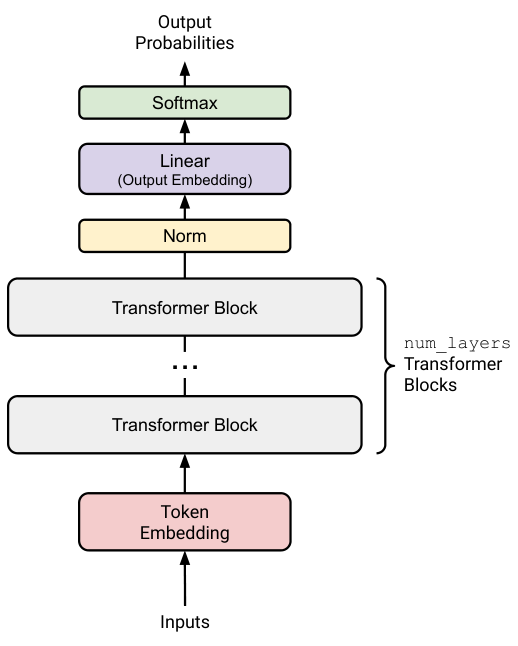
\includegraphics[width=0.88\linewidth]{figures/p13_v18.png}
  \caption{我们的 Transformer 语言模型总览。}
\end{minipage}\hfill
\begin{minipage}[t]{0.44\textwidth}
  \centering
  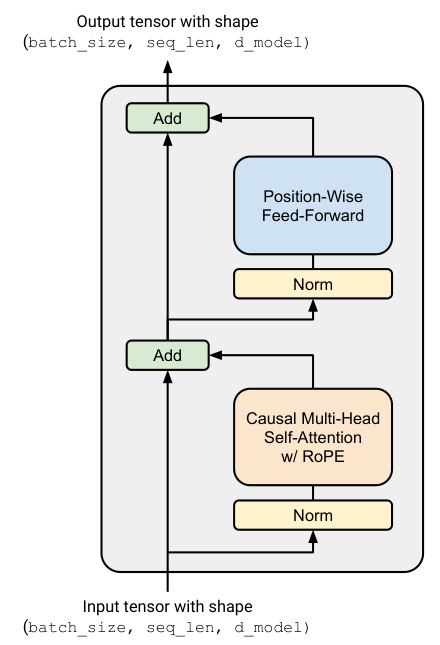
\includegraphics[width=0.82\linewidth]{figures/p13_v17.png}
  \caption{预归一化（pre-norm）Transformer 块。}
\end{minipage}
\end{figure}

\textbf{Token 嵌入}

第一步，Transformer 把（批量的）token ID 序列嵌入为一个向量序列，这些向量包含 token 身份的信息（图~1 中的红色方块）。

更具体地说，给定 token ID 序列，Transformer 语言模型用一个 token 嵌入层产生一个向量序列。每个嵌入层接收形状为 \tm{(batch\_size, sequence\_length)} 的整数张量，产生形状为 \tm{(batch\_size, sequence\_length, d\_model)} 的向量序列。

\textbf{预归一化（pre-norm）Transformer 块}

嵌入之后，这些激活值会经过若干结构完全相同的神经网络层。标准的 decoder-only Transformer 语言模型由 \tm{num\_layers} 个相同的层（通常称为 Transformer "块"）组成。每个 Transformer 块接收形状为 \tm{(batch\_size, sequence\_length, d\_model)} 的输入，并返回形状为 \tm{(batch\_size, sequence\_length, d\_model)} 的输出。每个块通过自注意力在序列维度上聚合信息，并通过前馈层对信息进行非线性变换。

经过 \tm{num\_layers} 个 Transformer 块之后，我们取出最终的激活值，把它们转换为词表上的一个分布。

我们将实现"预归一化（pre-norm）"Transformer 块（详见第 3.4 节），它还要求在最后一个 Transformer 块之后使用层归一化（layer normalization，下文详述），以确保其输出得到恰当的缩放。

这次归一化之后，我们用一个标准的可学习线性变换，把 Transformer 块的输出转换为预测的下一 token 的 logit（例如参见 A.~Radford et al.~[7] 的式~(2)）。

\subsection{附注：批处理、Einsum 与高效计算}

在整个 Transformer 中，我们要对许多"批状"输入重复执行同样的计算。举几个例子：

\begin{itemize}
  \item \textbf{批内元素}：我们对每个批元素施加相同的 Transformer 前向运算。
  \item \textbf{序列长度}：RMSNorm 和前馈网络这类"逐位置"运算对序列的每个位置做完全相同的处理。
  \item \textbf{注意力头}：注意力运算在多个注意力头上批量执行，构成"多头"注意力运算。
\end{itemize}

以一种既充分利用 GPU、又易读易懂的顺手方式执行这类运算，是很有价值的。许多 PyTorch 运算可以在张量开头接受额外的"批状"维度，并跨这些维度高效地重复/广播该运算。

例如，假设我们在做一个逐位置的批处理运算。我们有一个形状为 \tm{(batch\_size, sequence\_length, d\_model)} 的"数据张量" $D$，想把它与一个形状为 \tm{(d\_model, d\_model)} 的矩阵 $A$ 做批量向量--矩阵乘法。这时 \tm{D @ A} 会执行批量矩阵乘法——这是 PyTorch 中一个高效的原语，其中 \tm{(batch\_size, sequence\_length)} 这两个维度被批量化处理。

正因如此，最好假设你的函数可能会被传入额外的批状维度，并把这些维度放在 PyTorch 形状的开头。为了让张量能以这种方式批量处理，可能需要经过多步 \tm{view}、\tm{reshape} 和 \tm{transpose} 来塑形。这会有点痛苦，而且常常让人难以读懂代码在做什么、张量的形状是什么。

一个更顺手的选择是在 \tm{torch.einsum} 中使用 einsum 记法（einsum notation），或者使用 \tm{einops}、\tm{einx} 这类框架无关的库。两个关键运算是 \tm{einsum}（可以对任意维度的输入张量做张量缩并）和 \tm{rearrange}（可以重排、拼接和拆分任意维度）。事实证明，机器学习中几乎所有运算都是"维度搬运"与张量缩并的某种组合，再加上偶尔出现的（通常是逐点的）非线性函数。这意味着使用 einsum 记法可以让你的许多代码更易读、更灵活。

我们强烈建议本课程的同学学习并使用 einsum 记法。以前没接触过 einsum 记法的同学应该使用 \tm{einops}（见其文档）；已经熟悉 \tm{einops} 的同学应该学习更通用的 \tm{einx}（见其项目页面）。\footnote{值得注意的是，虽然 \tm{einops} 得到的支持非常广泛，但 \tm{einx} 没有经历那么多实战检验。如果你发现 \tm{einx} 有任何限制或 bug，请放心退回使用 \tm{einops} 加一些更普通的 PyTorch。}在我们提供的环境中，这两个包都已经安装好了。

下面我们给出一些使用 einsum 记法的例子。它们是 \tm{einops} 文档的补充，你应当先阅读其文档。

\subsubsection*{示例（\tm{einstein\_example1}）：用 \tm{einops.einsum} 做批量矩阵乘法}

\begin{lstlisting}
import torch
from einops import rearrange, einsum

## 基础实现
Y = D @ A.T
# 很难看出输入和输出的形状及其含义。
# D 和 A 可以是什么形状？其中是否存在意外的行为？

## Einsum 是自文档化且稳健的

#                        D                A   ->  Y

Y = einsum(D, A, "batch sequence d_in, d_out d_in -> batch sequence d_out")

## 或者，一个批处理版本：D 可以有任意前导维度，但 A 是受限的。
Y = einsum(D, A, "... d_in, d_out d_in -> ... d_out")
\end{lstlisting}

\subsubsection*{示例（\tm{einstein\_example2}）：用 \tm{einops.rearrange} 做广播运算}

我们有一批图像，想基于某个缩放因子为每张图像生成 10 个变暗版本：

\begin{lstlisting}
images = torch.randn(64, 128, 128, 3) # (batch, height, width, channel)
dim_by = torch.linspace(start=0.0, end=1.0, steps=10)

## 重塑并相乘
dim_value = rearrange(dim_by,    "dim_value          -> 1 dim_value 1 1 1")
images_rearr = rearrange(images, "b height width channel -> b 1 height width channel")
dimmed_images = images_rearr * dim_value

## 或者一步到位：
dimmed_images = einsum(
    images, dim_by,
    "batch height width channel, dim_value -> batch dim_value height width channel"
)
\end{lstlisting}

\subsubsection*{示例（\tm{einstein\_example3}）：用 \tm{einops.rearrange} 做像素混合}

假设我们有一批图像，表示为形状 \tm{(batch, height, width, channel)} 的张量，我们想对该图像的所有像素执行一个线性变换，但这个变换对每个通道应当相互独立。该线性变换表示为形状 \tm{(height * width, height * width)} 的矩阵 $B$。

\begin{lstlisting}
channels_last = torch.randn(64, 32, 32, 3)  # (batch, height, width, channel)
B = torch.randn(32*32, 32*32)

## 重排图像张量，以便在所有像素上混合
channels_last_flat = channels_last.view(
   -1, channels_last.size(1) * channels_last.size(2), channels_last.size(3)
)
channels_first_flat = channels_last_flat.transpose(1, 2)
channels_first_flat_transformed = channels_first_flat @ B.T
channels_last_flat_transformed = channels_first_flat_transformed.transpose(1, 2)
channels_last_transformed = channels_last_flat_transformed.view(*channels_last.shape)
\end{lstlisting}

改用 einops 则可以写成：

\begin{lstlisting}
height = width = 32
## rearrange 取代笨拙的 torch view + transpose
channels_first = rearrange(
    channels_last,
    "batch height width channel -> batch channel (height width)"
)
channels_first_transformed = einsum(
    channels_first, B,
    "batch channel pixel_in, pixel_out pixel_in -> batch channel pixel_out"
)
channels_last_transformed = rearrange(
    channels_first_transformed,
    "batch channel (height width) -> batch height width channel",
    height=height, width=width
)
\end{lstlisting}

或者，如果你想玩点花的：用 \tm{einx.dot}（\tm{einops.einsum} 的 einx 等价物）一气呵成

\begin{lstlisting}
height = width = 32
channels_last_transformed = einx.dot(
    "batch row_in col_in channel, (row_out col_out) (row_in col_in)"
    "-> batch row_out col_out channel",
    channels_last, B,
    col_in=width, col_out=width
)
\end{lstlisting}

这里的第一种实现可以通过在代码前后加注释来标明输入和输出的形状，但那样很笨拙，而且容易出 bug。使用 einsum 记法，文档即是实现！

Einsum 记法不仅能处理任意的输入批处理维度，还有一个关键好处：自文档化（self-documenting）。使用 einsum 记法编写的代码，能让输入和输出张量的相关形状一目了然。
